\documentclass[../main.tex]{subfiles}
\graphicspath{{\subfix{../images/}}}
\begin{document}

\subsubsection{Konstrukce eliminačního stromu}

Z prvků matice \matA.\\Pseudokód:

\begin{minipage}{0.95\linewidth}
\begin{verbatim}
    
for i = 1 ... n
    předek[i] = 0
    for k in {Soused i| index k< index i} 
        r=k
        while(předek[r]!= 0 and předek[r]!= i)
            r = předek[r]
        end while
        if(předek[r]==0) předek[r] = 1
    end k 
end i
\end{verbatim}    
\end{minipage}


\begin{example}
    \begin{equation*}
        \mathbb{A} = \begin{pmatrix}
            \times &&&\times&\\
            &\times&&&\times\\
            &&\times&\times&\times\\
            \times&&\times&\times&\\
            &\times&\times&&\times
        \end{pmatrix}
    \end{equation*}

    \begin{figure*}[H]
        \centering
        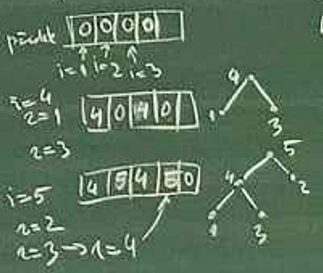
\includegraphics{images/26-10-elimstrompostup.png}
    \end{figure*}
\end{example}


\section{Řešení rovnic s řídkou SPD maticí}
Řešení $\mathbb{A} x = b $ s řídkou (SPD) maticí.

\begin{enumerate}
    \item Konstrukce eliminačního stromu
    \item Výpočet struktur řádků (sloupců) matice  $\mathbb{L}$
    \item Alokace paměti, vytvoření datových struktur $\mathbb{L}$
    \item Výpočet Choleského faktorizace $\mathbb{A}=\mathbb{L}\cdot\mathbb{L}^T$, respektive $\mathbb{A}=\mathbb{L}\cdot \mathbb{D} \cdot \mathbb{L}^T$
    \item 2 zpětné chody: $\mathbb{L} y = b, \mathbb{L}^T x = y$.
\end{enumerate}

V kroku 1-3 provádíme symbolickou faktorizaci, pracujeme se strukturou matice \matA.
V kroku 4 a 5 provádíme numerickou faktorizaci.

\begin{example}
    Zkoumejme vznik zaplnění u matice
    \begin{equation*}
        \mathbb{A} = \begin{pmatrix}
            \times&\times&\times&\times&\times&\times \\
            \times&\times&&&& \\
            \times&&\times&&& \\
            \times&&&\times&& \\
            \times&&&&\times& \\
            \times&&&&&\times 
        \end{pmatrix}
    \end{equation*}

    Po provedení jednoho kroku submaticového algoritmu dostaneme
    \begin{equation*}
        \begin{pmatrix}
            \times&\times&\times&\times&\times&\times \\
            \times&\times&\times&\times&\times&\times \\
            \times&\times&\times&\times&\times&\times \\
            \times&\times&\times&\times&\times&\times \\
            \times&\times&\times&\times&\times&\times \\
            \times&\times&\times&\times&\times&\times 
        \end{pmatrix}
    \end{equation*}
    tj. kompletně zaplněnou matici.

    Pokud ale prohodíme první a poslední řádek a sloupec matice \matA, tj.
    \begin{equation*}
        \begin{pmatrix}
            \times&&&&&\times \\
            &\times&&&&\times \\
            &&\times&&&\times \\
            &&&\times&&\times \\
            &&&&\times&\times \\
            \times&\times&\times&\times&\times&\times 
        \end{pmatrix}
    \end{equation*}
    tak v této matici zaplnění nevznikne.
\end{example}

Pokud chceme minimalizovat zaplnění, je možné permutovat řádky a sloupce matice \matA.

Vezměme permutační matici $\mathbb{P}$, pak místo $\mathbb{A}x=b$
řešíme \begin{equation*}
    \mathbb{P}\mathbb{A}\mathbb{P}^T y = \mathbb{P} b 
\end{equation*}


Omezujeme se na symetrické permutace
$\mathbb{A}=\mathbb{A}^T \implies \tilde{\mathbb{A}}= \mathbb{P}\mathbb{A}\mathbb{P}^T$ je také symetrická.
Diagonální prvky matice \matA zůstávájí na diagonále.

Ukažme souvislost s grafy matic. Nechť $\tilde{\mathbb{A}}= \mathbb{P}\mathbb{A}\mathbb{P}^T$. Pak platí
\begin{multline*}
    \tilde{a_{ij}} = a_{\varpi(i)\varpi(j)}\\
    \implies  (i,j)\in G(\tilde{\mathbb{A}}) \Leftrightarrow (\varpi(i), \varpi(j))\in G(\mathbb{A})\\
    \implies \text{Grafy } G(\mathbb{A}) \text{ a } G(\tilde{\mathbb{A}}) \text{ se liší jen číslováním vrcholů.} 
\end{multline*}

\begin{figure*}[H]
    \centering
    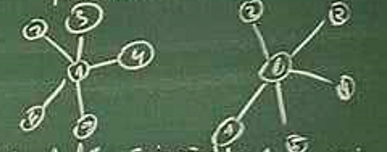
\includegraphics{images/26-10-cislovani.png}
\end{figure*}
 Číslování vrcholů určuje pořadí v eliminaci, tím vznikají rozdílné zaplnění.



Jak zvolit $\mathbb{P}$, aby se s maticí 
$\tilde{\mathbb{A}}= \mathbb{P}\mathbb{A}\mathbb{P}^T$
lépe pracovalo? Například aby 
\begin{enumerate}
    \item Matice $\tilde{\mathbb{A}}$ mělo lepší strukturu než $\mathbb{A}$
    \item $\mathbb{P}$ minimalizovala zaplnění
    \item $\tilde{\mathbb{A}}$ byla přizpůsobena počítačové architektuře (například možnost paralelizace)
\end{enumerate}

\subsection{Algoritmy pro vytvoření pásu, respektive profilu}

Označme $\forall i\in\hat{n}: f_i = \min\{j\in\hat{n} | a_{ij} \neq 0 \}$ toto označuje 
pozici 1. nenulového prvku v i-tém řádku.

Označme $\delta_i = i - f_i$, to nazvěme šířkou profilu v $i$-tém řádku 

Profilem \matA pak nazveme
\begin{equation*}
    Profil(\mathbb{A}) = \{(i,j)\in \hat{n}\times\hat{n}| i\geq j\geq i-\delta_i  \}
\end{equation*} 

Dále označme šířku pásu jako $\delta = \max_i \delta_i$.

Nakonec označme jako pás 
\begin{equation*}
    Pas(\mathbb{A}) = \left\{ (i,j)\in \hat{n}\times\hat{n} | i\geq j\geq i - \delta   \right\} 
\end{equation*}

Pro ilustraci 
\begin{figure*}[H]
    \centering
    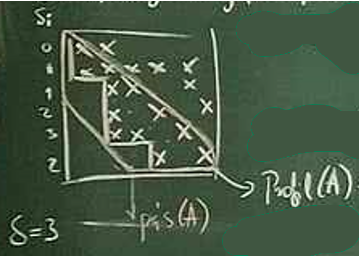
\includegraphics{images/26-10-profilpas.png}
\end{figure*}

Zaplnění vzniká jen uvnitř profilu.

\begin{example}
    \begin{figure*}[H]
        \centering
        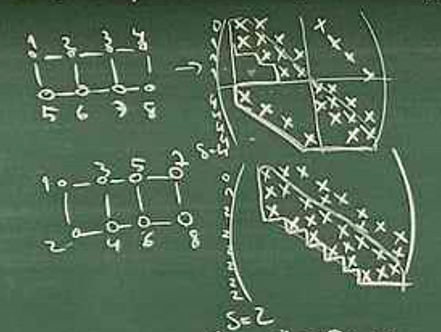
\includegraphics{images/26-10-zaplneni-uvnitr.png}
    \end{figure*}
    
Sousedi mají mít co nejbližší indexy, problém je u nepravidelných oblastí
\end{example}



\subsubsection{Algoritmus CMK (Cuthill, McKee)}
Číslování podle úrovní

\begin{enumerate}
    \item Zvol počáteční vrchol $x$, $L_0 = \{x\}$
    \item $L_1 = Adj(x)$
    \item $L_2 = Adj(L_1)\setminus(L_1 \cup \{x\})$
    \item[k.] $L_{k-1} = Adj(L_{k-2}) \setminus \bigcup_{j=0}^{k-1} L_j$  
    \item[End] Každý vrchol $G(\mathbb{A})$ je v některé z množin $L_1,L_2,\dots,L_p$, pak vrcholy čísluji nejprve v $L_0$, pak $L_1$, atd.   
\end{enumerate}

\begin{example}
    \begin{figure}[H]
        \centering
        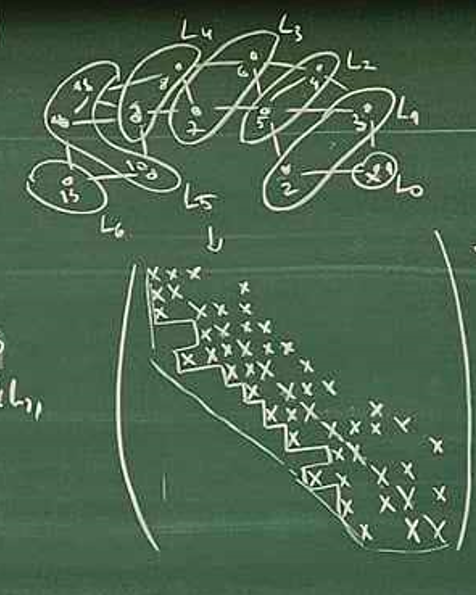
\includegraphics{images/26-10-CMK.png}
    \end{figure}
\end{example}

Sousedící prvky se liší maximálně o 1 úroveň, dostávají čísla po sobě, proto se vyváří pás.

Vzniká otázka jak zvolit počáteční vrchol.

Aby byl pás úzk, je třeba volit $x$ tak, aby vzniklo co nejvíce úrovní.

Průměr grafu označme $d(G)$, označujeme tak největší vzdálenost mezi 2 vrcholy v $G(A)$ měřenou délkou nejkratší cesty.

Vrcholy, mezi kterými existuje nejkratší cesta délky $d(G)$ se nazývají periferní, ty lze najít v $O(n^3)$ operací, to je složité proto hledáme pseudoperiferní vrcholy.

\subsubsection{Algoritmus GPS}

Nechť $x_0$ je startovní vrchol. Z CMK dostaneme $x_0 \rightarrow L_0,L_1, \dots, L_{K_1}$.

Zvolíme $x_1\in L_{K_1}$, z CMK opět $x_1 \rightarrow \tilde{L_0}, \tilde{L_1}, \dots, \tilde{L_{K_2}}$.

Pokud $K_2>K_1$ (tedy máme více úrovní) tak zvolme $x_2\in \tilde{L_{K_2}}$ a proces opakujeme, jinak algoritmus skončí a $x_1$ je pseudoperiferní vrchol.

Ukažme si ilustrační obrázek

\begin{example}
    \begin{figure}[H]
        \centering
        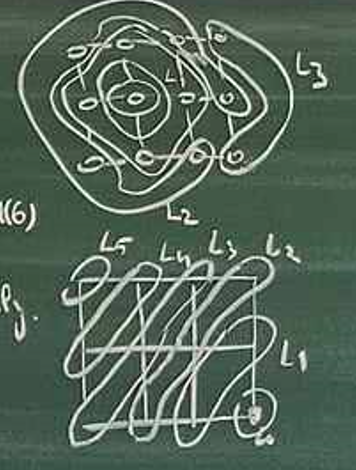
\includegraphics{images/26-10-GPS.png}
    \end{figure}
\end{example}

\begin{remark}
    Bylo zjištěno, že se někdy vyplatí po použití algoritmu CKM číslovat vrcholy opačně. Z toho plyne následující algoritmus
\end{remark}

\subsubsection{Algoritmus RCM (Reversed Cuthill McKee)}

\begin{enumerate}
    \item Najdi startovací vrchol $x_1$ pomocí GPS
    \item Pro $i=\hat{n}$, najdi všechny neočíslované sousedy $x_i$ a očísluj je (vzestupně podle stupně)
    \item Otoč číslování $y_i = x_{n+1-i}$ 
\end{enumerate}

Otočením číslování se někdy vylepší profil $(\sum_{i=1}^{n} \delta_i)$.\\
Šířka pásma se nezmění, dá se ukázat, že $\sum_{i=1}^{n} \delta_i$ se nezhorší. 



\end{document}